\chapter{Governança Territorial da Inovação e Políticas Públicas de CT\&I}
\label{cap:unid1_cap04}

\noindent\tagAV{AV1 (30\%)}\ \tagCritico

\vspace{6pt}

\begin{capObjetivos}
Ao concluir este capítulo, você deverá ser capaz de:
\begin{itemize}[leftmargin=1.4em, itemsep=3pt]
  \item Explicar a transição analítica da \textbf{Hélice Trípode} (Etzkowitz \& Leydesdorff) para os modelos de \textbf{Hélice Quádrupla} e \textbf{Hélice Quíntupla}, incorporando a sociedade civil e a transição socioecológica.
  \item Analisar o papel do \textbf{Estado Empreendedor} e das \textbf{Políticas Orientadas por Missões} (Mazzucato) no financiamento de risco tecnológico e na criação de mercados.
  \item Avaliar criticamente a eficácia de \textbf{habitats de inovação} (incubadoras, aceleradoras e parques tecnológicos), distinguindo ecossistemas enraizados de ``catedrais no deserto''.
  \item Interpretar e aplicar os principais instrumentos do \textbf{Marco Legal de CT\&I no Brasil} (Lei n.\textsuperscript{o} 10.973/2004, EC 85/2015, Lei n.\textsuperscript{o} 13.243/2016) e da \textbf{Lei do Bem} (Lei n.\textsuperscript{o} 11.196/2005).
  \item Formular críticas fundamentadas sobre a assimetria entre \textbf{socialização do risco e privatização dos ganhos} e sobre os riscos do \textbf{isomorfismo institucional} em políticas regionais.
\end{itemize}
\end{capObjetivos}

\begin{capRevisao}
No Capítulo~3, analisamos os Ecossistemas Empreendedores (Isenberg, Stam) e os Sistemas Regionais de Inovação (SRI), compreendendo como as cinco dimensões de proximidade de Boschma (cognitiva, organizacional, social, institucional e geográfica) condicionam a circulação de conhecimento. Neste Capítulo~4, damos um passo adiante para examinar \textbf{quem governa e quem financia} esses sistemas: as interações institucionais em hélice, os instrumentos jurídicos e fiscais de Ciência, Tecnologia e Inovação (CT\&I) e as tensões distributivas entre o setor público e o capital privado.
\end{capRevisao}

\etapa{3}{Fundamentação Teórica, Marco Legal e Modelagem}

\begin{boxSimbolo}[Vocabulário Conceitual e Símbolos do Capítulo]
\renewcommand{\arraystretch}{1.18}
\begin{tabular}{@{}p{2.4cm} p{12.0cm}@{}}
  $H_3, H_4, H_5$ & Modelos de Hélice Trípode, Quádrupla e Quíntupla de governança da inovação. \\
  $D_{P\&D}$ & Dispêndio total elegível em Pesquisa, Desenvolvimento e Inovação (em R\$). \\
  $\alpha_{excl}$ & Percentual de exclusão adicional na base de cálculo do IRPJ/CSLL (Lei do Bem). \\
  $\tau_{efetiva}$ & Alíquota tributária efetiva combinada de IRPJ e CSLL no regime de Lucro Real ($0{,}34$). \\
  $E_{LeiBem}$ & Economia fiscal líquida obtida via incentivos à P\&D da Lei n.\textsuperscript{o} 11.196/2005. \\
  $A_{pub}$ & Razão de alavancagem de investimento privado por unidade de recurso público ($I_{priv}/I_{pub}$). \\
  $E_{hab}$ & Índice de enraizamento territorial de um habitat de inovação ($0 \le E_{hab} \le 1$). \\
  ETEC / NIT & Encomenda Tecnológica / Núcleo de Inovação Tecnológica (Marco Legal de CT\&I). \\
\end{tabular}
\end{boxSimbolo}

\subsection{Da Hélice Trípode à Hélice Quádrupla e Quíntupla}

A governança da inovação territorial envolve a coordenação contínua de atores que operam sob lógicas institucionais distintas. Na formulação clássica de Henry Etzkowitz e Loet Leydesdorff, o modelo da \textbf{Hélice Trípode ($H_3$)} rompe com a visão linear de inovação (pesquisa básica $\to$ aplicada $\to$ mercado) ao propor uma dinâmica espiral de retroalimentação entre três esferas institucionais. Nessa arquitetura, a \textbf{Universidade} responde pela produção de conhecimento e formação avançada, a \textbf{Empresa} conduz a apropriação produtiva e a comercialização, e o \textbf{Governo} atua por meio da regulação, do fomento e do poder de compra. O elemento decisivo desse arranjo reside na sobreposição de papéis e na criação de organizações híbridas, de modo que universidades estruturam incubadoras e escritórios de transferência de tecnologia, empresas mantêm centros próprios de pesquisa e governos passam a operar como investidores de capital de risco.

\begin{boxConceito}[Evolução para a Hélice Quádrupla ($H_4$) e Quíntupla ($H_5$)]
Embora a Hélice Trípode explique com precisão a dinâmica de clusters industriais tradicionais, sua formulação original tende a negligenciar os usuários finais, os movimentos sociais e os limites ecológicos do território. Para superar essa restrição analítica, Carayannis e Campbell propuseram duas ampliações estruturais do modelo. A \textbf{Hélice Quádrupla ($H_4$)} incorpora a \textbf{sociedade civil organizada}, a cultura, a mídia e os usuários-cidadãos como quarta esfera de governança, fazendo com que a inovação seja coproduzida por meio de laboratórios vivos (\textit{living labs}), demandas sociais territorializadas e legitimação democrática das prioridades tecnológicas. Em um passo adicional, a \textbf{Hélice Quíntupla ($H_5$)} integra o \textbf{ambiente natural e a transição socioecológica} como quinta hélice, convertendo a crise climática, a conservação hídrica e a biodiversidade em vetores centrais que orientam e restringem a P\&D territorial.
\end{boxConceito}

Quando essas cinco esferas se articulam no território, as decisões tecnológicas deixam de responder apenas a critérios de eficiência industrial isolada e passam a incorporar legitimidade social e sustentabilidade ambiental. A Figura~\ref{fig:helice_quintupla} esquematiza essa arquitetura integrada, destacando os fluxos de conhecimento e governança entre Universidade, Empresa, Estado, Sociedade Civil e Transição Socioecológica.

\begin{figure}[H]
  \centering
  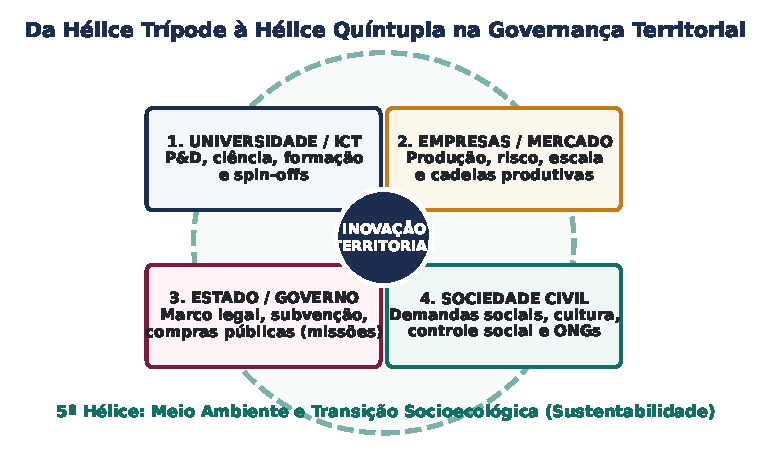
\includegraphics[width=0.90\textwidth]{figures/fig04_helice_quintupla.pdf}
  \caption{Modelo integrado da Hélice Quíntupla: articulação entre Universidade, Empresa, Estado, Sociedade Civil e Transição Socioecológica na governança territorial da inovação.}
  \label{fig:helice_quintupla}
\end{figure}

\subsection{Estado Empreendedor e Políticas Orientadas por Missões}

Na teoria econômica neoclássica convencional, a intervenção estatal em CT\&I justifica-se apenas para corrigir \textit{falhas de mercado}, como as externalidades positivas da pesquisa básica e as assimetrias de informação. Mariana Mazzucato contesta essa visão minimalista ao evidenciar que as grandes ondas tecnológicas contemporâneas (internet, GPS, telas sensíveis ao toque, biotecnologia e energias renováveis) dependeram de um \textbf{Estado Empreendedor}, isto é, de um setor público disposto a assumir a \textbf{incerteza radical} nos estágios iniciais da inovação, quando o capital privado e o \textit{venture capital} ainda se recusam a entrar devido ao longo prazo de maturação e ao elevado risco técnico.

Complementarmente, as \textbf{Políticas Orientadas por Missões} propõem organizar os instrumentos de CT\&I em torno de desafios territoriais concretos e mensuráveis, como a descarbonização de cadeias produtivas, a segurança hídrica no Semiárido ou a bioeconomia amazônica. Ao definir problemas públicos específicos como eixo coordenador, o poder público substitui a distribuição indiferenciada de subsídios horizontais por metas estratégicas com direcionalidade clara, mobilizando múltiplos setores e atores locais em torno de soluções verificáveis.

\subsection{Habitats de Inovação: Sucesso Territorial vs. ``Catedrais no Deserto''}

Incubadoras de empresas, aceleradoras e parques tecnológicos constituem \textbf{habitats de inovação} destinados a reduzir custos de transação e acelerar a maturação de empreendimentos intensivos em conhecimento. Contudo, a literatura de economia regional alerta para o fenômeno das \textbf{``catedrais no deserto''}, caracterizado por grandes complexos imobiliários financiados com recursos públicos em regiões desprovidas de base produtiva aderente, massa crítica de pesquisadores ou demanda empresarial local.

Sem densidade cognitiva nem encadeamentos produtivos regionais, as empresas graduadas nesses espaços tendem a migrar para metrópoles em busca de mercado e fornecedores especializados, drenando o investimento público municipal. Para evitar esse isolamento, o parque tecnológico ou a incubadora exige \textbf{enraizamento territorial}, que se efetiva mediante conexão orgânica com as cadeias produtivas locais, presença de âncoras demandantes e mecanismos concretos de retenção de talentos e empresas no próprio território.

\subsection{Marco Legal de CT\&I no Brasil e Lei do Bem}

O arcabouço jurídico brasileiro de incentivo à inovação evoluiu nas últimas duas décadas para reduzir a insegurança jurídica na interação entre universidades e empresas. O ponto de inflexão iniciou-se com a \textbf{Lei de Inovação (Lei n.\textsuperscript{o} 10.973/2004)}, que instituiu os Núcleos de Inovação Tecnológica (NITs) nas Instituições Científicas, Tecnológicas e de Inovação (ICTs), regulamentou o compartilhamento de laboratórios públicos e autorizou a subvenção econômica direta a empresas. Na sequência, a \textbf{Lei do Bem (Lei n.\textsuperscript{o} 11.196/2005, Cap. III)} criou incentivos fiscais automáticos, dispensando aprovação prévia de projeto e exigindo apenas prestação de contas posterior ao MCTI, para empresas tributadas pelo \textbf{Lucro Real} que realizem dispêndios em P\&D\&I, permitindo exclusão adicional de 60\% a 100\% desses gastos na apuração do IRPJ e da CSLL.

Esse conjunto normativo foi aprofundado pela \textbf{Emenda Constitucional n.\textsuperscript{o} 85/2015} e pelo \textbf{Novo Marco Legal de CT\&I (Lei n.\textsuperscript{o} 13.243/2016, regulamentada pelo Decreto n.\textsuperscript{o} 9.283/2018)}, que constitucionalizou o Sistema Nacional de CT\&I e simplificou procedimentos de compras para pesquisa. Além disso, o Novo Marco autorizou a participação minoritária do Estado no capital de empresas de base tecnológica e consolidou a \textbf{Encomenda Tecnológica (ETEC)}, instrumento que permite ao poder público contratar diretamente o esforço de P\&D de soluções com risco tecnológico, mesmo quando o resultado final ainda é incerto.

\begin{boxConceito}[Contraponto Crítico: Socialização do Risco e Isomorfismo Institucional]
Duas patologias recorrentes comprometem a eficácia das políticas territoriais de CT\&I. A primeira consiste na \textbf{socialização do risco com privatização dos ganhos}, situação em que o Estado financia a pesquisa básica e absorve a incerteza inicial, mas entrega a propriedade intelectual e os lucros futuros integralmente ao setor privado sem cláusulas de retorno, tais como \textit{royalties}, participação acionária, licenciamento acessível ou contrapartidas territoriais. A segunda patologia refere-se ao \textbf{isomorfismo institucional}, isto é, à tendência de gestores públicos replicarem acriticamente modelos de regiões centrais (como o Vale do Silício ou Cambridge) em territórios periféricos ou semiáridos, ignorando a estrutura produtiva local e gerando estruturas burocráticas ociosas.
\end{boxConceito}

\begin{boxFormula}[Modelagem Quantitativa da Lei do Bem e do Enraizamento de Habitats]
\textbf{1. Economia Fiscal Efetiva pela Lei do Bem (Lucro Real):}
Para uma empresa com lucro tributável sujeito à alíquota combinada de IRPJ (15\% + adicional de 10\%) e CSLL (9\%), totalizando $\tau_{efetiva} = 0{,}34$, a economia tributária adicional decorrente da exclusão incentivada de dispêndios em P\&D é:
\[
E_{LeiBem} = D_{P\&D} \times \alpha_{excl} \times \tau_{efetiva}
\]
onde $\alpha_{excl} = 0{,}60$ (regra geral), podendo receber acréscimo de $+0{,}20$ se houver incremento superior a 5\% no número de pesquisadores dedicados exclusivamente à P\&D (totalizando $0{,}80$), ou $+0{,}10$ se o incremento for de até 5\%, além de $+0{,}20$ caso haja patente concedida ou cultivar registrada (chegando a $\alpha_{excl} = 1{,}00$).

\vspace{4pt}
\textbf{2. Alavancagem de Fomento Público e Índice de Enraizamento de Habitat:}
\[
A_{pub} = \frac{I_{priv}}{I_{pub}} \qquad \text{e} \qquad E_{hab} = \left(\frac{E_{locais}}{E_{total}}\right) \times \left(\frac{C_{locais}}{C_{total}}\right)
\]
Em que $E_{locais}/E_{total}$ é a proporção de empresas graduadas que permanecem sediadas no território após 3 anos, e $C_{locais}/C_{total}$ é a fração de compras de insumos e serviços tecnológicos contratados junto a fornecedores regionais.
\end{boxFormula}

\etapa{4}{Exemplos Resolvidos e Estudos de Caso Comentados}

\begin{boxExemplo}{4.1}{Mapeamento da Hélice Quíntupla no Semiárido Baiano}
\passoEnunciado{Um consórcio intermunicipal do Semiárido baiano pretende estruturar um programa de inovação para a cadeia da caprinocultura leiteira e forragicultura adaptada à seca, evitando o modelo tradicional de pacotes tecnológicos importados.}
\passoDados{Participam: (i) universidade pública estadual com laboratório de genética e nutrição animal; (ii) 45 pequenas agroindústrias e laticínios regionais; (iii) secretaria estadual de ciência e tecnologia e banco regional de fomento; (iv) associações de agricultores familiares e sindicatos rurais; (v) plano estadual de convivência com o Semiárido e combate à desertificação.}
\passoPedido{Classificar cada ator segundo o modelo da Hélice Quíntupla ($H_5$) e identificar o risco caso a quarta e a quinta hélices sejam excluídas da governança.}
\passoMetodo{Aplicação analítica do modelo de Carayannis, Barth e Campbell ($H_5$), mapeando as cinco esferas institucionais e suas interfaces de retroalimentação.}
\passoContas{
Mapeamento das cinco hélices no território:
\begin{itemize}[leftmargin=1.4em, itemsep=2pt]
  \item \textbf{Hélice 1 (Academia):} Universidade estadual (P\&D em manejo forrageiro e melhoramento genético).
  \item \textbf{Hélice 2 (Empresa):} Laticínios e agroindústrias locais (processamento, logística e comercialização).
  \item \textbf{Hélice 3 (Estado):} Secretaria de CT\&I e banco de fomento (crédito direcionado, assistência técnica e compras públicas institucionais).
  \item \textbf{Hélice 4 (Sociedade Civil):} Associações de agricultores familiares (validação participativa das tecnologias e legitimidade social).
  \item \textbf{Hélice 5 (Transição Socioecológica):} Agenda de convivência com o Semiárido (uso racional de água, conservação da Caatinga e energia solar rural).
\end{itemize}
}
\passoResposta{Todas as cinco hélices estão representadas. A exclusão da Hélice 4 geraria rejeição por inadequação cultural e produtiva; a exclusão da Hélice 5 induziria sobrepastejo e esgotamento hídrico.}
\passoVerificacao{O diagnóstico demonstra coerência territorial: no Semiárido, a sustentabilidade ecológica (Hélice 5) e a organização comunitária (Hélice 4) são condições de viabilidade econômica, e não meros apêndices.}
\end{boxExemplo}

\begin{boxExemplo}{4.2}{Cálculo de Benefício Fiscal pela Lei do Bem (Lei n.\textsuperscript{o} 11.196/2005)}
\passoEnunciado{Uma empresa baiana de biotecnologia agrícola, tributada pelo Lucro Real e com lucro fiscal positivo, investiu em pesquisa para bioinsumos adaptados ao cerrado e ao semiárido.}
\passoDados{Dispêndio elegível em P\&D no ano-base: $D_{P\&D} = \reais{1.200.000,00}$. A empresa ampliou sua equipe exclusiva de pesquisadores em $8\%$ em relação ao ano anterior (acima do gatilho de $5\%$), não possuindo ainda patente concedida no período. Alíquota combinada efetiva de IRPJ e CSLL: $\tau_{efetiva} = 0{,}34$.}
\passoPedido{Calcular o percentual total de exclusão adicional ($\alpha_{excl}$), a economia fiscal líquida ($E_{LeiBem}$) e o custo líquido efetivo do investimento em P\&D após o incentivo.}
\passoMetodo{Aplicação direta da equação de economia fiscal da Lei do Bem: $E_{LeiBem} = D_{P\&D} \times \alpha_{excl} \times \tau_{efetiva}$.}
\passoContas{
1. Percentual de exclusão adicional:
\[
\alpha_{excl} = 0{,}60\ (\text{base}) + 0{,}20\ (\text{incremento de pesquisadores } > 5\%) = 0{,}80\ (80\%)
\]
2. Economia fiscal adicional (além da dedução normal como despesa operacional):
\[
E_{LeiBem} = 1.200.000 \times 0{,}80 \times 0{,}34 = 960.000 \times 0{,}34 = \reais{326.400,00}
\]
3. Note-se que, como despesa operacional dedutível, o dispêndio já reduz o imposto em $1.200.000 \times 0{,}34 = \reais{408.000,00}$. Somando a dedução normal à exclusão incentivada ($E_{LeiBem}$), a redução tributária total atinge $\reais{734.400,00}$, reduzindo o custo líquido desembolsado pela empresa para $\reais{465.600,00}$ ($38{,}8\%$ do valor original).
}
\passoResposta{Exclusão adicional $\alpha_{excl} = 80\%$; economia fiscal incentivada $E_{LeiBem} = \reais{326.400,00}$.}
\passoVerificacao{O resultado reflete o limite legal da Lei do Bem para empresas no Lucro Real com lucro tributável. Em empresas iniciantes (\textit{startups}) no Simples Nacional ou em prejuízo fiscal, esse incentivo não é utilizável, exigindo outros instrumentos como subvenção econômica.}
\end{boxExemplo}

\begin{boxExemplo}{4.3}{Diagnóstico de ``Catedral no Deserto'' em Parques Tecnológicos}
\passoEnunciado{Dois municípios do interior brasileiro inauguraram parques tecnológicos há cinco anos. O gestor estadual precisa comparar o desempenho territorial dos dois habitats para decidir a renovação de aportes públicos.}
\passoDados{
\textbf{Parque A:} Investimento público acumulado $I_{pub} = \reais{40\text{ milhões}}$; investimento privado atraído $I_{priv} = \reais{12\text{ milhões}}$; de $20$ empresas graduadas, apenas $4$ permaneceram no território ($E_{locais} = 4$); fração de compras locais de serviços e insumos $C_{locais}/C_{total} = 0{,}15$.\\
\textbf{Parque B:} $I_{pub} = \reais{25\text{ milhões}}$; $I_{priv} = \reais{50\text{ milhões}}$; de $22$ empresas graduadas, $18$ permaneceram no território; fração de compras locais $C_{locais}/C_{total} = 0{,}65$.
}
\passoPedido{Calcular a razão de alavancagem $A_{pub}$ e o índice de enraizamento $E_{hab}$ de ambos os parques, diagnosticando qual deles se configura como ``catedral no deserto''.}
\passoMetodo{Cálculo comparativo via $A_{pub} = I_{priv}/I_{pub}$ e $E_{hab} = (E_{locais}/E_{total}) \times (C_{locais}/C_{total})$.}
\passoContas{
\textbf{Parque A:}
\[
A_{pub, A} = \frac{12}{40} = 0{,}30 \qquad \text{e} \qquad E_{hab, A} = \left(\frac{4}{20}\right) \times 0{,}15 = 0{,}20 \times 0{,}15 = 0{,}030\ (3{,}0\%)
\]
\textbf{Parque B:}
\[
A_{pub, B} = \frac{50}{25} = 2{,}00 \qquad \text{e} \qquad E_{hab, B} = \left(\frac{18}{22}\right) \times 0{,}65 \approx 0{,}8182 \times 0{,}65 \approx 0{,}5318\ (53{,}2\%)
\]
}
\passoResposta{O Parque A apresenta baixa alavancagem ($0{,}30$) e enraizamento residual ($E_{hab} = 3{,}0\%$), caracterizando-se como ``catedral no deserto''. O Parque B alavanca $2{,}00$ reais privados por real público e retém mais de metade do efeito multiplicador ($E_{hab} = 53{,}2\%$).}
\passoVerificacao{A diferença expressiva mostra que infraestrutura física sem encadeamento produtivo local gera fuga de empresas graduadas para metrópoles, drenando o investimento público municipal.}
\end{boxExemplo}

\begin{boxExemplo}{4.4}{Encomenda Tecnológica (ETEC) para Segurança Hídrica}
\passoEnunciado{Um município do Polígono das Secas enfrenta salinização de poços artesianos. As tecnologias comerciais disponíveis têm custo energético proibitivo para comunidades rurais isoladas. A prefeitura decide utilizar o instrumento de Encomenda Tecnológica (ETEC), previsto na Lei n.\textsuperscript{o} 13.243/2016.}
\passoDados{Orçamento total de P\&D estimado para desenvolver um protótipo de dessalinizador solar de baixo custo: $\reais{2.000.000,00}$. Pelo contrato de compartilhamento de risco tecnológico, o poder público remunera $80\%$ dos custos de desenvolvimento conforme entregas de marcos técnicos e a \textit{startup} contratada assume $20\%$ como risco próprio, recebendo direito à encomenda em escala caso atinja a meta de eficiência.}
\passoPedido{Determinar o aporte máximo de risco assumido pelo Estado e pela \textit{startup}, explicando por que a licitação convencional por menor preço falharia nesse caso.}
\passoMetodo{Análise jurídico-econômica da ETEC (art. 20 da Lei n.\textsuperscript{o} 10.973/2004, alterado pela Lei n.\textsuperscript{o} 13.243/2016) e repartição contratual de risco.}
\passoContas{
1. Parcela de risco tecnológico assumida pelo ente público:
\[
R_{Estado} = 2.000.000 \times 0{,}80 = \reais{1.600.000,00}
\]
2. Parcela de contrapartida/risco assumida pela \textit{startup}:
\[
R_{Startup} = 2.000.000 \times 0{,}20 = \reais{400.000,00}
\]
Na licitação tradicional por menor preço, pressupõe-se que o objeto já exista pronto no mercado. Como a solução demanda P\&D com risco de insucesso técnico, nenhum fornecedor sério assumiria preço fixo sem margem proibitiva; a ETEC permite pagar pelo esforço de pesquisa validado por marcos, mesmo diante de incerteza.
}
\passoResposta{O Estado assume $\reais{1.600.000,00}$ ($80\%$) e a \textit{startup} assume $\reais{400.000,00}$ ($20\%$) do risco de desenvolvimento, viabilizando uma missão pública territorial.}
\passoVerificacao{Esse desenho concretiza o conceito de Estado Empreendedor e compras públicas para inovação, vinculando o gasto público a uma demanda real do território.}
\end{boxExemplo}

\begin{boxExemplo}{4.5}{Socialização do Risco vs. Privatização dos Ganhos}
\passoEnunciado{Uma agência pública de fomento aportou capital não reembolsável em uma empresa privada para o desenvolvimento de um software de monitoramento agrícola por satélite.}
\passoDados{Aporte público a fundo perdido: $I_{pub} = \reais{5.000.000,00}$. Após a validação da tecnologia, a empresa alcançou receita acumulada de $\reais{60.000.000,00}$ em 5 anos e Valor Presente Líquido privado de $\reais{25.000.000,00}$. Compare o Cenário 1 (contrato sem cláusula de retorno financeiro ao fundo público) com o Cenário 2 (contrato com cláusula de \textit{royalty} contingente ao sucesso comercial de $3\%$ sobre a receita bruta).}
\passoPedido{Calcular o retorno financeiro direto ao fundo público e a taxa de recuperação do aporte público em ambos os cenários.}
\passoMetodo{Cálculo do fluxo de retorno contratual ($R_{pub} = r \times \text{Receita}$) e da razão de recuperação ($R_{pub}/I_{pub}$).}
\passoContas{
\textbf{Cenário 1 (sem cláusula de retorno):}
\[
R_{pub, 1} = \reais{0,00} \implies \text{Recuperação} = 0\%
\]
\textbf{Cenário 2 (com \textit{royalty} contingente de $3\%$ sobre $\reais{60\text{ milhões}}$):}
\[
R_{pub, 2} = 60.000.000 \times 0{,}03 = \reais{1.800.000,00} \implies \text{Recuperação} = \frac{1.800.000}{5.000.000} = 0{,}36\ (36\%)
\]
}
\passoResposta{No Cenário 1 ocorre privatização integral dos ganhos ($0\%$ de retorno direto ao fundo). No Cenário 2, o fundo recupera $\reais{1.800.000,00}$ ($36\%$ do aporte), permitindo reinvestimento em novas missões territoriais sem inviabilizar o lucro privado.}
\passoVerificacao{Mecanismos como \textit{royalties} contingentes ao sucesso ou participação acionária pública (\textit{equity}) mitigam a assimetria apontada por Mazzucato, mantendo o fundo de inovação sustentável.}
\end{boxExemplo}

\etapa{5}{Armadilhas Conceituais e Erros Mais Comuns}

\begin{boxErro}[Erro 1: Confundir Hélice Quádrupla/Quíntupla com ``Mais Burocracia'']
Incluir sociedade civil ($H_4$) e transição socioecológica ($H_5$) não significa criar conselhos meramente consultivos e lentos. Significa incorporar a \textbf{demanda social} e a \textbf{restrição ecológica} na fase de concepção tecnológica, evitando que o projeto fracasse por rejeição comunitária ou inviabilidade ambiental na fase de difusão.
\end{boxErro}

\begin{boxErro}[Erro 2: Aplicar a Lei do Bem a Empresas do Simples Nacional ou Lucro Presumido]
Um erro técnico recorrente em projetos de consultoria é prometer economia fiscal via Lei n.\textsuperscript{o} 11.196/2005 para \textit{startups} recém-criadas. A Lei do Bem exige obrigatoriamente apuração pelo \textbf{Lucro Real} e existência de lucro fiscal no exercício; empresas em prejuízo ou no Simples Nacional não usufruem desse benefício.
\end{boxErro}

\begin{boxErro}[Erro 3: Reduzir o Estado Empreendedor a ``Gasto Público Sem Critério'']
Defender o Estado Empreendedor não equivale a aprovar subsídios incondicionais. A proposta de Mazzucato exige \textbf{direcionalidade por missões}, monitoramento de metas técnicas e mecanismos de compartilhamento de retornos quando o risco assumido pelo setor público gera lucros extraordinários.
\end{boxErro}

\begin{boxErro}[Erro 4: Replicar Parques Tecnológicos por Isomorfismo Institucional]
Construir prédios espelhados com salas de \textit{coworking} em municípios sem massa crítica científica nem vocação produtiva articulada cria apenas custos fixos de manutenção. O hardware (infraestrutura) nunca substitui o software institucional (confiança, demanda qualificada e capital humano).
\end{boxErro}

\etapa{6}{Exercícios Propostos (Básicos, Intermediários e Objetivos)}

\textbf{Parte A, Exercícios Básicos (Conceituação e Identificação)}

\textbf{1.} Diferencie, em até cinco linhas, o papel da Universidade e do Estado no modelo linear de inovação em comparação ao modelo da Hélice Trípode ($H_3$).
\espacoResolucao[1.8cm]

\textbf{2.} Explique por que a transição da Hélice Trípode ($H_3$) para a Hélice Quíntupla ($H_5$) é estratégica para territórios com alta vulnerabilidade climática, como o Semiárido nordestino.
\espacoResolucao[1.8cm]

\textbf{3.} Cite três instrumentos jurídicos introduzidos ou fortalecidos pelo Novo Marco Legal de CT\&I (Lei n.\textsuperscript{o} 13.243/2016) que facilitam a cooperação entre ICTs públicas e empresas.
\espacoResolucao[1.8cm]

\textbf{4.} Uma empresa optante pelo Lucro Presumido investiu $\reais{500.000,00}$ em P\&D e solicita o benefício fiscal da Lei do Bem. O pedido é juridicamente válido? Justifique.
\espacoResolucao[1.8cm]

\textbf{5.} Defina o conceito de ``catedral no deserto'' aplicado a parques tecnológicos e indique duas condições necessárias para evitá-la.
\espacoResolucao[1.8cm]

\textbf{Parte B, Exercícios Intermediários (Modelagem e Análise Quantitativa)}

\textbf{6.} Uma indústria farmacêutica no Lucro Real investiu $D_{P\&D} = \reais{2.500.000,00}$ em pesquisa de fitoterápicos nativos. A empresa não aumentou seu quadro de pesquisadores, mas obteve uma patente concedida no exercício, elevando $\alpha_{excl}$ para $0{,}80$ ($60\%$ base + $20\%$ patente). Com $\tau_{efetiva} = 0{,}34$, calcule a economia fiscal incentivada ($E_{LeiBem}$).
\espacoResolucao[2.0cm]

\textbf{7.} Um polo de inovação recebeu $\reais{15\text{ milhões}}$ de recursos públicos e atraiu $\reais{45\text{ milhões}}$ de investimento privado. Das $30$ empresas incubadas e graduadas, $21$ permanecem operando no município e realizam $50\%$ de suas compras de serviços na região. Calcule $A_{pub}$ e $E_{hab}$ e interprete o resultado.
\espacoResolucao[2.0cm]

\textbf{8.} Analise uma política pública estadual que concede subvenção econômica integral ($100\%$ a fundo perdido) para empresas estrangeiras instalarem centros de dados no território, sem exigência de contratação de pesquisadores locais nem transferência tecnológica para universidades regionais. Avalie à luz dos conceitos de \textit{enraizamento} e \textit{socialização do risco}.
\espacoResolucao[2.0cm]

\textbf{9.} Uma prefeitura deseja contratar o desenvolvimento de um sistema de alerta inteligente de enchentes com sensores ainda não disponíveis comercialmente. Compare os prós e contras de utilizar um pregão eletrônico tradicional versus uma Encomenda Tecnológica (ETEC).
\espacoResolucao[2.0cm]

\textbf{10.} Elabore o desenho sintético de uma \textbf{Política Orientada por Missões} para o seu território (ou para a Região Metropolitana de Feira de Santana), especificando: (a) o grande desafio territorial, (b) a missão mensurável com prazo, e (c) os instrumentos de fomento e poder de compra mobilizados.
\espacoResolucao[2.0cm]

\textbf{Parte C, Questões Objetivas (Estilo Exame / Concurso, A a E)}

\textbf{11.} Sobre a evolução dos modelos de Hélice de inovação (Etzkowitz, Leydesdorff, Carayannis e Campbell), assinale a alternativa \textbf{correta}:
\begin{alternativas}
  \item A Hélice Trípode exclui o setor público da dinâmica inovativa, restringindo-o à cobrança de tributos.
  \item A Hélice Quádrupla substitui as universidades pela mídia digital como principal produtora de conhecimento científico.
  \item A Hélice Quíntupla integra o ambiente natural e a transição socioecológica como dimensões estruturantes da governança da inovação.
  \item Na Hélice Trípode, as esferas institucionais atuam de forma estanque, sendo vedada a criação de organizações híbridas como os NITs.
  \item O modelo de Hélice Quíntupla aplica-se exclusivamente a países de alta renda com matriz energética nuclear.
\end{alternativas}

\textbf{12.} No debate econômico proposto por Mariana Mazzucato em \textit{O Estado Empreendedor}, a atuação estatal nas fases iniciais de tecnologias disruptivas caracteriza-se principalmente por:
\begin{alternativas}
  \item Limitar-se à correção de falhas de mercado após a consolidação comercial da tecnologia pelo capital privado.
  \item Assumir a incerteza radical por meio de financiamento paciente e compras públicas estratégicas, moldando e criando novos mercados.
  \item Substituir integralmente o empreendedorismo privado em todas as etapas de comercialização varejista.
  \item Eliminar a necessidade de proteção de propriedade intelectual em favor da desregulamentação tributária absoluta.
  \item Concentrar recursos apenas em empréstimos de curto prazo com taxas de juros superiores às de mercado.
\end{alternativas}

\textbf{13.} Em relação ao Marco Legal de CT\&I no Brasil (Lei n.\textsuperscript{o} 10.973/2004, EC 85/2015 e Lei n.\textsuperscript{o} 13.243/2016) e à Lei do Bem (Lei n.\textsuperscript{o} 11.196/2005), é \textbf{correto} afirmar que:
\begin{alternativas}
  \item A Lei do Bem permite que microempresas do Simples Nacional deduzam até $100\%$ de seus gastos de P\&D no imposto de renda.
  \item A Encomenda Tecnológica (ETEC) só pode ser utilizada para a compra de equipamentos padronizados de prateleira pelo critério de menor preço.
  \item Os Núcleos de Inovação Tecnológica (NITs) são proibidos por lei de negociar contratos de licenciamento de patentes com o setor privado.
  \item A Lei n.\textsuperscript{o} 13.243/2016 ampliou a segurança jurídica para o compartilhamento de laboratórios de ICTs públicas com empresas e para a realização de ETECs em projetos com risco tecnológico.
  \item A EC 85/2015 retirou da Constituição Federal a competência dos estados e municípios para legislar e fomentar sistemas locais de inovação.
\end{alternativas}

\textbf{14.} Uma empresa tributada pelo Lucro Real realiza dispêndio elegível de $\reais{1.000.000,00}$ em P\&D, enquadrando-se na exclusão adicional básica de $60\%$ da Lei do Bem ($\alpha_{excl} = 0{,}60$). Considerando $\tau_{efetiva} = 34\%$, o valor da economia fiscal adicional ($E_{LeiBem}$) proporcionada exclusivamente pelo incentivo da Lei do Bem é de:
\begin{alternativas}
  \item $\reais{170.000,00}$
  \item $\reais{204.000,00}$
  \item $\reais{340.000,00}$
  \item $\reais{544.000,00}$
  \item $\reais{600.000,00}$
\end{alternativas}

\textbf{15.} O fenômeno do \textit{isomorfismo institucional} em políticas regionais de CT\&I manifesta-se quando:
\begin{alternativas}
  \item Um território adapta instrumentos de fomento às suas vocações produtivas endógenas e à sua biodiversidade.
  \item Agências de fomento exigem cláusulas de retorno público (\textit{royalties}) proporcionais ao risco tecnológico assumido.
  \item Gestores locais copiam formatos institucionais de ecossistemas hegemônicos (como parques tecnológicos genéricos) sem aderência à base econômica e social do território.
  \item Cooperativas agrícolas utilizam a Encomenda Tecnológica para desenvolver máquinas adaptadas à agricultura familiar.
  \item Universidades regionais reorganizam seus NITs para priorizar demandas de cadeias produtivas locais.
\end{alternativas}

\etapa{7}{Questões Autorais Estilo Pós-Graduação e Concursos}

\textbf{16. (Estilo ENADE / Pós-Graduação em Políticas Públicas)} Analise criticamente a seguinte afirmação: \textit{``A criação de um parque tecnológico de alto padrão arquitetônico e a concessão de isenções fiscais genéricas são condições suficientes para transformar uma região periférica em um polo de inovação dinâmica.''} Fundamente sua resposta com os conceitos de Hélice Quíntupla, ``catedrais no deserto'' e isomorfismo institucional.
\espacoResolucao[2.2cm]

\textbf{17. (Estilo Concurso para Analista em CT\&I, FINEP/FAPs)} Uma fundação estadual de amparo à pesquisa (FAP) financiou a fundo perdido o desenvolvimento de um novo bioinseticida em parceria entre uma universidade estadual e uma empresa privada. Cinco anos depois, a empresa vendeu a patente para uma multinacional e desativou a planta fabril no estado. Proponha três mecanismos contratuais e de governança, amparados pelo Marco Legal de CT\&I e pela abordagem de Mazzucato, que poderiam ter evitado a socialização do risco com privatização integral dos ganhos e perda territorial.
\espacoResolucao[2.2cm]

\textbf{18. (Estilo Mestrado Profissional, PPGPT/UEFS)} Um município baiano pretende estruturar um sistema local de inovação para a cadeia da mandioca e derivados (farinha especial, fécula biodegradável e bioembalagens). Redija uma proposta de governança em Hélice Quíntupla indicando: (i) os atores de cada uma das cinco hélices; (ii) um instrumento do Marco Legal de CT\&I aplicável; e (iii) dois indicadores quantitativos para monitorar o enraizamento territorial do programa.
\espacoResolucao[2.2cm]

\begin{boxDica}[Contraponto Crítico e Preparação para a AV1 (30\%)]
Ao analisar políticas públicas de CT\&I no seu fichamento crítico ou seminário da \textbf{AV1}, evite avaliações puramente descritivas (``a lei existe e cria incentivos''). Pergunte sempre: \textbf{quem acessa o instrumento} (grandes empresas no Lucro Real ou cooperativas e \textit{startups} locais?), \textbf{quem assume o risco inicial} e \textbf{qual parcela do valor gerado permanece retida no território}.
\end{boxDica}

\clearpage
\etapa{8}{Gabarito Comentado dos 18 Exercícios}

\begin{boxGabarito}[Respostas Comentadas: Capítulo 4]
\textbf{1.} No modelo linear, a universidade gera ciência básica isoladamente e o Estado apenas financia pesquisas sem interação direta. Na Hélice Trípode ($H_3$), Universidade, Empresa e Estado sobrepõem esferas, criando organizações híbridas (NITs, incubadoras, fundos de risco) em interação contínua.

\textbf{2.} A Hélice Quíntupla incorpora a sociedade civil ($H_4$) e a transição socioecológica ($H_5$). No Semiárido, inovações que ignoram o balanço hídrico, a conservação da Caatinga e a organização comunitária tendem à degradação ambiental e à baixa adoção social.

\textbf{3.} Entre os principais instrumentos: (i) Encomenda Tecnológica (ETEC); (ii) compartilhamento de laboratórios e infraestrutura de ICTs com empresas; (iii) permissão para participação minoritária do poder público no capital social de empresas inovadoras e simplificação da gestão financeira pelos NITs.

\textbf{4.} Não é válido. O benefício fiscal da Lei do Bem (Cap. III da Lei n.\textsuperscript{o} 11.196/2005) restringe-se a pessoas jurídicas tributadas pelo regime do \textbf{Lucro Real} que apurem lucro fiscal no período.

\textbf{5.} ``Catedral no deserto'' é um habitat de inovação (ex.: parque tecnológico) com alto investimento imobiliário público, porém desconectado do tecido produtivo local. Para evitá-la, exige-se demanda empresarial/pública aderente e articulação densa com ICTs e cadeias locais.

\textbf{6.} $E_{LeiBem} = 2.500.000 \times 0{,}80 \times 0{,}34 = \reais{680.000,00}$.

\textbf{7.} $A_{pub} = 45 / 15 = 3{,}00$ (cada real público alavancou $\reais{3,00}$ privados). $E_{hab} = (21/30) \times 0{,}50 = 0{,}70 \times 0{,}50 = 0{,}35$ ($35\%$). O habitat apresenta forte alavancagem privada e retenção territorial moderada-alta.

\textbf{8.} A política promove socialização do risco (subsídio integral público) com baixa retenção territorial: centros de dados operam com pouca mão de obra local e, sem contrapartida de P\&D regional ou transferência tecnológica, funcionam como enclaves desconectados do território.

\textbf{9.} O pregão eletrônico exige especificação fechada e produto pronto, inviabilizando soluções inéditas ou induzindo sobrepreço pelo risco. A ETEC permite contratar o esforço de P\&D com risco tecnológico compartilhado e marcos de entrega, ainda que exija maior capacidade técnica de fiscalização do gestor público.

\textbf{10.} Resposta aberta estruturada: deve definir um desafio territorial concreto (ex.: gestão de resíduos sólidos industriais ou eficiência hídrica), uma meta quantificável com prazo (ex.: reduzir em $40\%$ o descarte inadequado em 5 anos) e combinar fomento à P\&D com compras públicas (ETEC).

\textbf{11. (C)} A Hélice Quíntupla amplia a Hélice Quádrupla ao inserir o ambiente natural e a sustentabilidade socioecológica no centro da governança inovativa.

\textbf{12. (B)} Mazzucato demonstra que o Estado Empreendedor assume a incerteza radical e cria mercados por meio de financiamento paciente e missões, não se limitando a corrigir falhas residuais.

\textbf{13. (D)} A Lei n.\textsuperscript{o} 13.243/2016 consolidou a segurança jurídica para compartilhamento de infraestrutura de ICTs e para a contratação via ETEC. (A) exige Lucro Real; (B) ETEC é para risco tecnológico; (C) NITs têm essa atribuição; (E) EC 85 fortaleceu competências subnacionais.

\textbf{14. (B)} $E_{LeiBem} = 1.000.000 \times 0{,}60 \times 0{,}34 = \reais{204.000,00}$.

\textbf{15. (C)} Isomorfismo institucional ocorre quando se copiam modelos externos (como parques tecnológicos genéricos) sem adequação à estrutura produtiva e institucional local.

\textbf{16.} A afirmação é falsa. Infraestrutura física e isenções genéricas não criam densidade cognitiva nem demanda qualificada; sem conexão com a base produtiva, com a sociedade civil ($H_4$) e com a sustentabilidade ($H_5$), reproduz-se o isomorfismo institucional e criam-se ``catedrais no deserto''.

\textbf{17.} Três mecanismos: (i) cláusula de \textit{royalties} contingentes ao sucesso comercial revertidos ao fundo estadual; (ii) cláusula de permanência produtiva territorial ou preferência de licenciamento local em caso de transferência de controle; (iii) participação acionária minoritária ou bônus de subscrição pública, além de retenção de co-titularidade da PI pela ICT pública via NIT.

\textbf{18.} Academia: universidade/instituto federal (biotecnologia de amidos e bioplásticos); Empresa: casas de farinha modernizadas e indústrias de embalagens; Estado: prefeitura/governo estadual (ETEC ou subvenção FAP); Sociedade Civil: cooperativas de mandiocultores; Transição Socioecológica: substituição de plásticos fósseis e aproveitamento da manipueira. Indicadores sugeridos: $A_{pub}$ e $E_{hab}$ (ou taxa de retenção de valor local).
\end{boxGabarito}

\begin{boxResumo}
\begin{itemize}[leftmargin=1.4em, itemsep=3pt]
  \item A governança territorial evoluiu da \textbf{Hélice Trípode} (Universidade--Empresa--Estado) para a \textbf{Quádrupla} (+ Sociedade Civil) e a \textbf{Quíntupla} (+ Transição Socioecológica).
  \item O \textbf{Estado Empreendedor} assume incerteza radical e orienta políticas por \textbf{missões}, evitando subsídios sem direcionalidade.
  \item No Brasil, o \textbf{Marco Legal de CT\&I} (Leis 10.973/2004 e 13.243/2016) e a \textbf{Lei do Bem} (11.196/2005, exclusiva do Lucro Real) oferecem instrumentos complementares de cooperação e fomento.
  \item Políticas territoriais devem evitar o \textbf{isomorfismo institucional} (``catedrais no deserto'') e a assimetria entre \textbf{socialização do risco e privatização dos ganhos}.
\end{itemize}
\end{boxResumo}

\begin{boxTeste}
Julgue os itens a seguir como Verdadeiros (\V) ou Falsos (\F):
\begin{enumerate}[leftmargin=1.6em, itemsep=3pt]
  \item (\quad) A Hélice Quíntupla acrescenta o ambiente natural e a transição socioecológica como eixo estruturante da inovação territorial.
  \item (\quad) Empresas enquadradas no Simples Nacional podem utilizar a exclusão adicional de $60\%$ a $100\%$ da Lei do Bem no cálculo de seus tributos.
  \item (\quad) A Encomenda Tecnológica (ETEC) permite que o poder público contrate diretamente soluções com risco tecnológico em que o resultado final ainda é incerto.
  \item (\quad) O índice de enraizamento $E_{hab}$ será baixo mesmo que um parque tecnológico tenha alto investimento público, caso as empresas graduadas migrem para fora do território.
\end{enumerate}
\textbf{Gabarito do Checkpoint:} 1. \V \quad 2. \F \text{ (exige Lucro Real)} \quad 3. \V \quad 4. \V
\end{boxTeste}
